\documentclass[letterpaper,12pt]{article}
\usepackage[english]{babel}							%For internationalization
\usepackage[utf8]{inputenc}							%For character encoding
\usepackage{amsmath}								%For mathematical typesetting
\usepackage{amssymb}
\usepackage{graphicx}								%For handling graphics
\usepackage[top=1in, bottom=.75in, left=1in, right=1in]{geometry}	%Sets required thesis margins

\title{Galerkin Method: Mathe-magic?\\ A concise-ish explanation}
\author{Josh Bevan}
\date{\today}

\newcommand{\be}{\begin{equation}}
\newcommand{\ben}[1]{\begin{equation}\label{#1}}
\newcommand{\ee}{\end{equation}}

\begin{document}
\maketitle
\section{Example PDE}

\begin{figure}
\centering
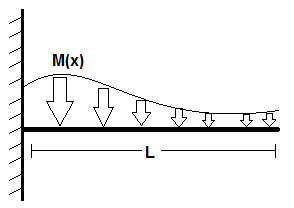
\includegraphics{Beam.PNG}
\caption{\label{fig:Beam}An elastic 1-D beam subject to arbitrary moment, M(x).}
\end{figure}

Imagine you would like to solve for the deflection of an elastic 1-D beam subject to an external moment (see Figure~\ref{fig:Beam}), we know from solid mechanics the deflection u is given by:
\be\frac{d^2u(x)}{dx^2} = M(x)\ee

where for simplicity we assume E and I are constant across the beam, and EI=1.

Note that if $u(x)$ is the correct solution, then of course:

\be\frac{d^2u(x)}{dx^2}- M(x)=0\ee


However the whole reason we are interested in finding a numerical solution is that we don't have the exact analytical solution $u(x)$; instead we attempt to find some approximate answer, let's call it $\bar{u}(x)$. It is important to note that our approximate solution will not satisfy our original PDE (if it did, then we should stop right there as it's an exact answer!), instead we will be left with some error, the residual:
\be \frac{d^2\bar{u}(x)}{dx^2}- M(x)=R(x)\ee

It seems reasonable that a "good" approximate solution is one that attempts to minimize the residual in some fashion; the smaller the residual, the closer to the exact solution we are. The question becomes: how do we decide what the best approximate solution is? We need to decide on some mathematical statement that quantifies how close the approximate solution is to the exact solution. To do this we need to talk briefly about vector spaces, inner products, and orthogonality.

\section{A Mathematical Interlude}
The concept of a "vector", at least in the geometric sense, is a familiar one. You might have something like $\overrightarrow{v_1}=(2,3)$ which we interpret to mean a vector in 2-D with components 2 and 3 in the x and y directions. This vector exists on the x-y plane, more accurately we would call this "Euclidean space" or $\mathbb{R}^2$. We can extend all of the concepts of  Euclidean space to a more general object called a \textit{vector space}. Just like in a Euclidean space we have: vectors, a measure of distance, and several other features we will use shortly.

\subsection{Vector Bases}
We represent our vector $\overrightarrow{v_1}$ in Euclidean space by means of \textit{bases}, for $\mathbb{R}^2$ the usual ones are $\hat{\imath}=(1,0)$ and $\hat{\jmath}=(0,1)$. We can see then that really our $\overrightarrow{v_1}$ can be expressed as $\overrightarrow{v_1}=2\hat{\imath} + 3\hat{\jmath}$. In general we can imagine representing any vector in N-dimensional space as:
\be\overrightarrow{v}=\sum^N_{i=1} a_i\hat{\phi}_i\ee
where each $\hat{\phi}_i$ is the basis for each dimension $i$. We say that any vector in a vector space is a \textit{linear combination} of bases in that space. Note that vector spaces can be \textit{finite dimensional}; so for instance the 3-D Euclidean basis $\hat{k}=(0,0,1)$ does not appear in $\mathbb{R}^2$ space but is contained in $\mathbb{R}^3$ space.

We can extend this concept to a general vector space, and allow things other than geometric vectors to be bases. Imagine we choose monomials like $3x^4$ to be our basis. This would give us a vector space of polynomials. The "dimension" of our polynomial space then is the highest order polynomial we can represent, e.g.
\be f \in \mathbb{P}^N  \qquad f=\sum^N_{i=1} a_ix^{i-1}\ee
All the concepts of geometric vectors apply to the general vector space (like our polynomial space). Four important ones are the inner product, orthogonality, norm, and projection.

\subsection{Inner Product}
For geometric vectors, the inner product is the familiar dot product:
\be a \cdot b = a_x b_x + a_y b_y + a_z b_z + \ldots = \sum^N_{i=1} a_i b_i\ee
where the last expression is for a N-dimensional geometric vector.

For the type of vector spaces used in Galerkin methods, the inner product is defined as
\be \int_a^b f(x)g(x) dx \ee
Here our polynomial space we created is also included, so we can talk about the inner product of two polynomials over some interval $x \in (a,b)$. It is common to simplify the inner product notation as $\langle a | b \rangle$. Note that the inner product for functions seems as if it turned a finite sum of terms into an integral; we shall see a similar behavior for 
%----------------------------------
\subsection{Orthogonality}
\begin{figure}
\centering
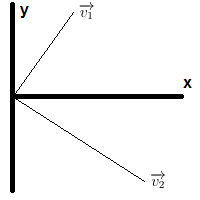
\includegraphics{OrthoVect.PNG}
\caption{\label{fig:OrthoVect}Two orthogonal geometric vectors. Their dot product (inner product) is zero.}
\end{figure}

For geometric vectors we say two vectors are orthogonal if their dot product is zero. Orthogonal vectors are perpendicular in Euclidean space.
\be \overrightarrow{v_1}=(2,3), \overrightarrow{v_2}=(6,-4) \ee
\be \overrightarrow{v_1} \cdot \overrightarrow{v_2} = (2*6) + (3*-4) = 0 \ee
A graphical representation of this can be seen in Figure~\ref{fig:OrthoVect}.

As you might expect, two vectors in a general vector space are orthogonal if their inner product is zero. So in the space we use for the Galerkin method, two functions are orthogonal if:
\be \int_a^b f(x)g(x) dx =0 \ee
As an example, $sin(x)$ and $cos(x)$ are orthogonal in the domain $x \in (-1, 1)$
\be \int_{-1}^1 sin(x)cos(x) dx = -\frac{1}{2} cos^2(x)\Big\rvert_{-1}^{1} = 0\ee
%----------------------------------
\subsection{Vector Norm}
A vector norm is a measure of the "size" of a vector. For geometric vectors the $\ell^2$ norm is simply the length of the vector. So our the $\ell^2$ norm of our friend $\overrightarrow{v_1}$ is  
\be \Vert\overrightarrow{v_1}\Vert_2 = \sqrt{2^2+3^2} \approx 3.61 \ee
or more generally
\be \Vert\overrightarrow{v}\Vert_2 = \sqrt{\sum_i^N a_i^2} \ee
We can talk about the "distance" between two vectors by looking at the norm of the difference between the two vectors, with the distance between the vector and itself of course being zero.

As we saw for the inner product, the sum for the geometric vector case turns into an integral for functions, so the $L^2$ form for functions is:
\be \Vert f \Vert_2 = \sqrt{\int_a^b f(x)^2 dx} = \sqrt{\langle f | f \rangle} \ee
%----------------------------------
\subsection{Projection}
\begin{figure}
\centering
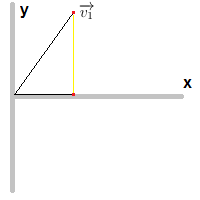
\includegraphics{Proj.PNG}
\caption{\label{fig:Proj}The projection of a vector onto a lower dimensional space.}
\end{figure}

For geometric vectors projection has an intuitive meaning, we "project" a vector onto another space. For instance we could project our buddy $\overrightarrow{v_1}=(2,3)$ who lives in  $\mathbb{R}^2$ onto a lower dimensional space  $\mathbb{R}^1$. It is trivial to calculate the projection in this case: $\overrightarrow{v'_1}=(2)$. But how would we generalize this?

When we are projecting $\overrightarrow{v_1}$ what we are actually doing is 

\end{document}